\chapter{Evaluation}
The goal of this paragraph is to assure that the changes we made to AutoWDS basic actually improved its performance.
Due to extent this work is aimed at, it was not feasible to implement all the systems of the related solutions on this field on a common environment
to get a fair assessment for each work. For this the overview papers on this area like \cite{overview_caa} may serve its purpose.
The following subsections will mainly focus on the comparison between AutoWDS basic and the extended version. Also we were not able to evaluate the performance gains
of some metrics like the survival path feature since the current implementation of AutoWDS only uses network bridges to connect the networks and no real routing infrastructure.
Due to this restriction only we are limited to spanning trees for the network since otherwise the STP would force shutdown the redundant links to eliminate
circles in the topology.
\section{Test Arrangement}
Since the main goal is to increase overall throughput performance as described in the requirements analysis, our basic evaluation approach is
to find by how much we were able to increase this metric. Therefore we ran both systems under equal circumstances with various settings and multiple runs
and compared its capacities.
  \subsection{Physical Infrastructure}
    For the test arrangement we used the following hardware:
      11 Accesspoints, one WLC and two Switches among those
      \begin{itemize}
       \item 3 x LANCOM L322agn dual Wireless \cite{lancom}
       \item 3 x LANCOM L-452agn dual Wireless
       \item 6 x Hirschmann OpenBAT-R
       \item 1 x LANCOM WLC-4100
       \item 2 x LANCOM GS-2352P
      \end{itemize}
      running on developer firmware version 9.0 with special extensions for our purpose not included in the mainline.
      We deployed them at a typical office environment as depicted in the figure.
      Only omnidirectional antennas for the accesspoints were used for this setup. As we had to connect each of the accesspoints also
      per cable to the monitoring station and power grid in order to route traffic through them and the network they're spanning,
      we could not set them further apart.
      Increasing the distance between the single APs would have lead to a sparser network topology and so the hidden station problem would have occured
      more often. Thus the actual interference would have gone up, since with a lower Signal to Noise ratio the APs would not be able to recognize each others 
      transmissions as those and categorize it as interference instead of applying CSMA/CD, leading to more corrupt packets.
      We were able to simulate this problem with a reduced transmit-power,
      but even on the lowest setting most of the accesspoints were able to receive each others beacons. With this limitation kept in mind we expect
      the gap between the two scenarios in the following results to be even greater.
      Since this test was conducted at a research facility for wireless LAN devices, especially the 2.4Ghz band was quite heavily utilized as you will notice
      in the performance charts.
    \begin{figure}[h!]
      \centering
      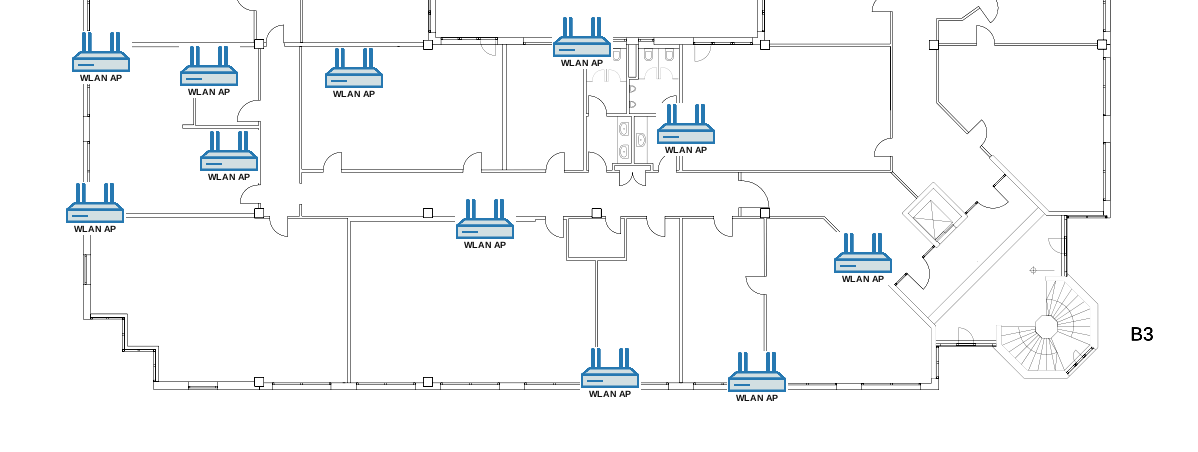
\includegraphics[width=1\columnwidth]{figures/Lancom-flur-withaps}
      \caption{Physical arrangement of accesspoints in a typical office complex spread over an area of rougly 15m x 40m}
      \label{fig:2ndfloor}
    \end{figure}
  \subsection{Network Infrastructure}
    The basic approach for measuring the throughput is to attach traffic generators to the accesspoints and make those send as much broadcast traffic to all
    other stations which are part of this network and therefore saturate the throughput capabilities of the network. The idea behind this setup is to simulate real 
    end-device-clients attached to the accesspoints, where each client has its own ip address and therefore mac- address and table. This constraint and also the additional effort
    to implement a custom traffic generator in LCOS are the reason for this approach.
    \begin{figure}[h!]
      \centerline{
	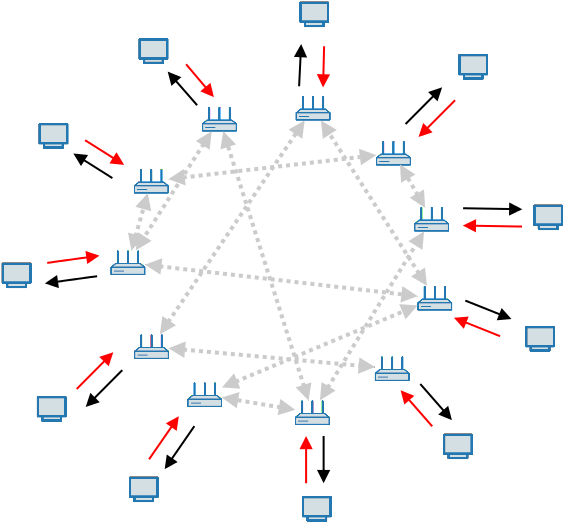
\includegraphics[width=0.6\textwidth]{figures/testsetup_logic}
	\caption{Example for the logical arrangement of accesspoints with systems attached by cable, which generate broadcast traffic that is routed through the 
	wireless network spanned by the accesspoints.}
      }
      \label{fig:testsetup_logic}
    \end{figure}
    
    \begin{figure}[h!]
      \centerline{
	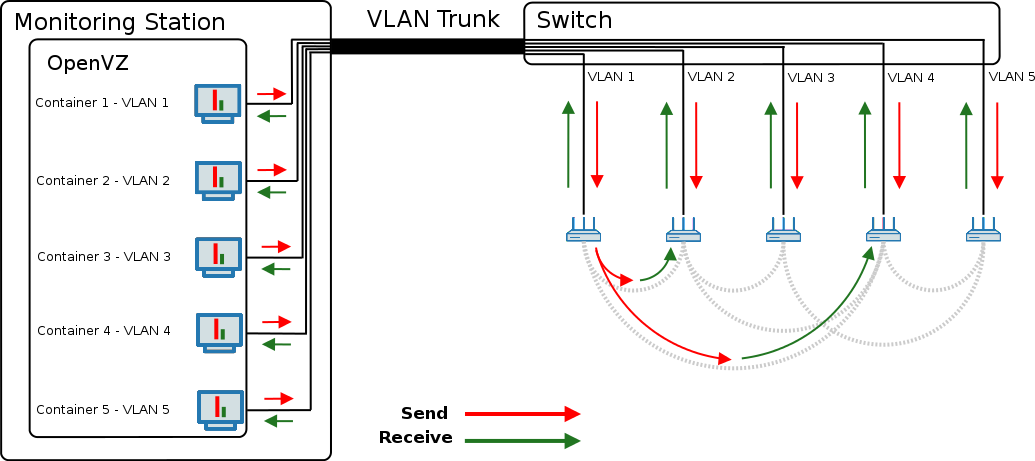
\includegraphics[width=0.8\textwidth]{figures/testsetup_openvz}%
	\caption{Implementation of the test arrangement with available hardware.}
      }
      \label{fig:testsetup_openvz}
    \end{figure}
    We simulated the traffic generating systems with OpenVZ \cite{openvz} on one Host with a VLAN for each system. The VLAN infrstructure is completely transparent
    to the VZ containers and the accesspoints since the monitoring stations encapsulates all frames before sending if over the VLAN Trunk to the switch, which again 
    decapsulates the frames before sending them to the accesspoints.
    To generate the traffic we used IPerf \cite{iperf} on the attached systems in UDP mode with a datarate of 1Mbit per second for a total of 10 Minutes.
    Since we could not directly send UDP frames to broadcast addresses with iperf, we ran multiple instances of iperf with different target ip addresses.
    Although 1Mbit for each stream may not seem much, but after multiplying it with the number of targets and the up- and downstreams the effective rate results in
    1Mbit * 12 * 2 = 24Mbit/s for each accesspoint. As we will see later on this will turn out to be enough to completely saturate the wireless network but still within
    the capabilities of the used Gigabit Ethernet to get the data to the accesspoints, as 24Mbit/s * 11 = 264Mbit/s does not exceed the 1000Mbit/s VLAN Trunk connection
    as possible bottleneck.
    \begin{listing}[h!]
      \begin{lstlisting}
iperf -u -c 172.16.40.2* -t 600 -b 1M
      \end{lstlisting}
      \caption{IPerf's parameters to generate the traffic.}
      \label{lst:iperf}
    \end{listing}

\section{Metrics}
  \subsection{Test Duration}
     Each testcase was run for a total of 10 minutes as this should be enough to transgress any temporary effects. To get status snapshots we querried the accesspoints
     every 7 seconds for their state, which includes the bytes transferred and received so far. We did not query them more often since this could have 
     affected the accesspoints transfer performance as reading its internal tables and sending the results back means additional stress.
  \subsection{Channelusage}
    For AutoWDS basic we configured the Accesspoints to only use the following sets of Channels:
    \begin{itemize}
     \item 1 (2.4 GHz only)
     \item 36 (5GHz only)
    \end{itemize}
    For the extended version of AutoWDS we used the following channels as input for the allocation algorithm: 
    \begin{itemize}
     \item 1,6,11 (2.4 GHz only)
     \item 36,40,44 (5GHz only)
     \item 1,6,11,36,40,44 (2.4/5 Ghz mixed)
    \end{itemize}
    
    \begin{figure}[h!]
      \centerline{
	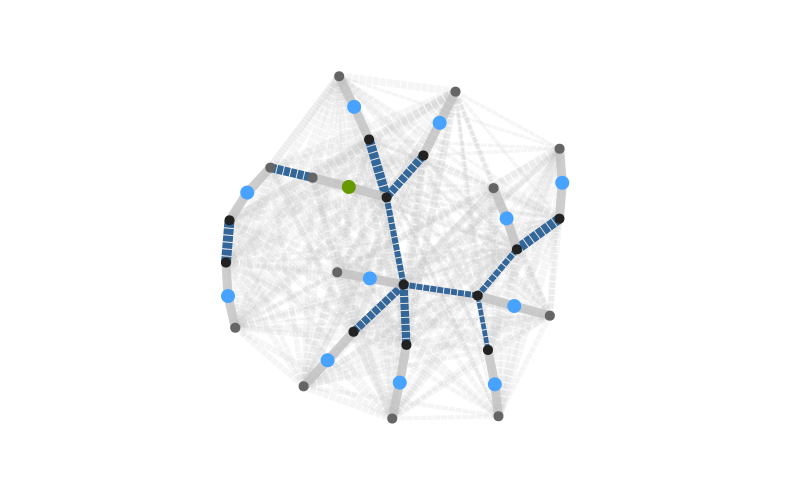
\includegraphics[width=0.7\textwidth]{figures/topo_chan_1}%
	\caption{Topology of the testnetwork with only channel 1 used. Different colors indicate different channels}
      }
      \label{fig:topo_chan_1}
    \end{figure}
    
    \begin{figure}[h!]
      \centerline{
	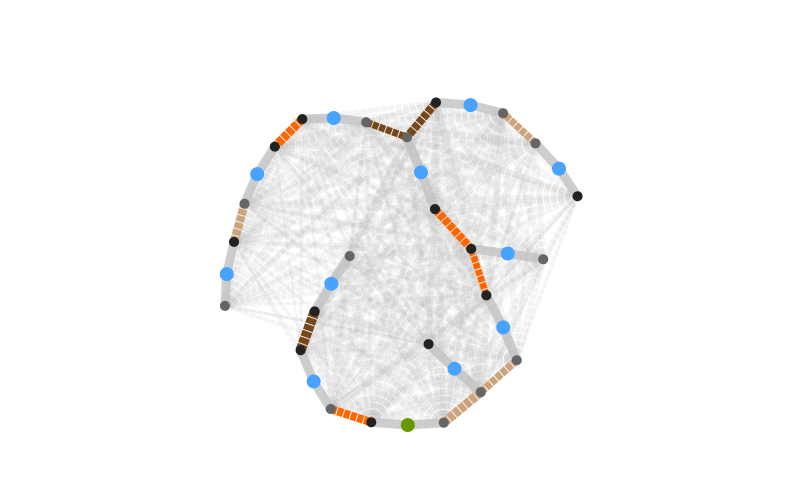
\includegraphics[width=0.7\textwidth]{figures/topo_chan_36_40_44}%
	\caption{Topology of the testnetwork with only channel 36,40,44 being used.}
      }
      \label{fig:topo_chan_36_40_44}
    \end{figure}

    \begin{figure}[h!]
      \centerline{
	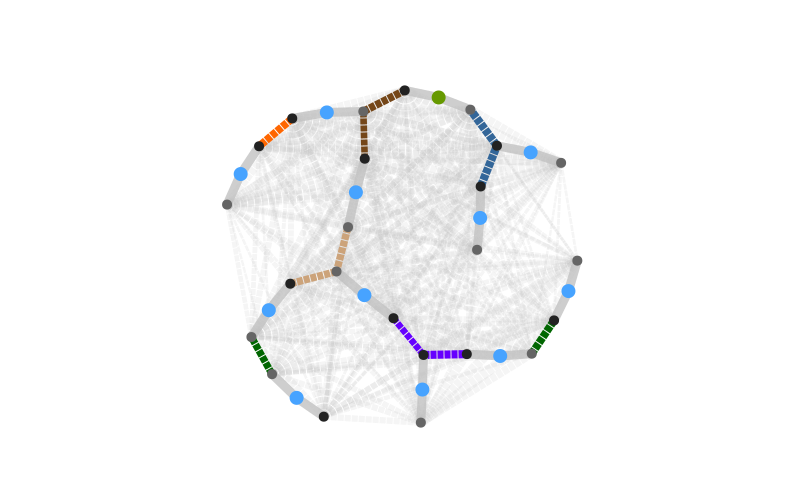
\includegraphics[width=0.7\textwidth]{figures/topo_chan_1_6_11_36_40_44}%
	\caption{Topology of the testnetwork with only channel 1,6,11,36,40,44 being used.}
      }
      \label{fig:topo_chan_1_6_11_36_40_44}
    \end{figure}
    
    \subsection{Characteristics}
    Due to the exceptional utilization of the 2.4 Ghz band in the area around the test arrangement, we had to carefully chose time and day
    for running the tests. We noticed a significant drop in radio usage for weekends and evenings and were able to schedule our tests in those timeframes.
    We additionally ran the testcases with two different settings to simulate the hidden station problem. Therefore we first set the radios to full power 
    resulting in a high connectivity between the nodes and on a second run decreased the transmit power as much as possbile to get a network with a smaller degree
    of interconnectivity.
    
\section{Results}
  We would expect a significant increase of data that has been able to transmit due to the usage of multiple collision domains the same one could
  expect by comparing a network hub, which has essentially just one collision domain and a network switch which has multiple domains and does not have
  to wait until the medium is free for sending again. The second source for an increased throughput would be the number of packets that could be received
  without errors due to interference. Up next we take a look at the actual measurement results.
    
  \subsection{Description}
    \begin{figure}[h!]
      \centerline{
	\includegraphics[width=0.62\textwidth]{figures/TestDataDiagramme/20/rx_bytes}%
	\includegraphics[width=0.38\textwidth]{figures/TestDataDiagramme/20/rx_bytes_boxplot}%
      }
      \caption{Received bytes with decreased antenna transmit power}
      \label{fig:rx20_bytes}
    \end{figure}
    
    \begin{figure}[h!]
      \centerline{
	\includegraphics[width=0.62\textwidth]{figures/TestDataDiagramme/3/rx_bytes}%
	\includegraphics[width=0.38\textwidth]{figures/TestDataDiagramme/3/rx_bytes_boxplot}%
      }
      \caption{Received bytes with full transmit power}
      \label{fig:rx3_bytes}
    \end{figure}
    
    Analyzing the successfully received bytes for the low power \ref{fig:rx20_bytes} and high power \ref{fig:rx3_bytes} setup we recognize noticeable differences for 
    each channel-assigning.
    
      \begin{itemize}
	\item The base scenarios where only one channel was utilized performe the worst within a range of 0.5 to 1.5Mbit/s on average per accesspoint.
	  Using three channels gives roughly three times the throughput (2.5 - 5Mbit/s for 2.4Ghz and 2.5 - 5Mbit/s for 5Ghz) compared to the baseline.
	  Utilizing up to 6 Channels shows the best results with an effective throughput of 5.5 - 9Mbit/s. Note that the gain for the 6 channel setup 
	  is still linear as it provides roughly 6 times the throughput of the baseline.
	\item We further discern that the high transmit power setup outperformes the low power setup by a factor of two with an even more noticeable difference.
	\item With slight variations for the high-power 3/2.4Ghz setup the rates are also rather constant.
	\item Besides the high-power 1/5Ghz setup we realize 5Ghz's superiority over the 2.4Ghz band.
      \end{itemize}

    \begin{figure}[h!]
      \centerline{
	\includegraphics[width=0.56\textwidth]{figures/TestDataDiagramme/3/recpackerr}%
	\includegraphics[width=0.44\textwidth]{figures/TestDataDiagramme/3/recpackerr_boxplot}%
	\caption{Ratio of successfully received packets to packets containing errors for reduced transmit power scenario}
      }
      \label{fig:3recpackerr}
    \end{figure}
    \begin{figure}[h!]
      \centerline{
	\includegraphics[width=0.56\textwidth]{figures/TestDataDiagramme/20/recpackerr}%
	\includegraphics[width=0.44\textwidth]{figures/TestDataDiagramme/20/recpackerr_boxplot}%
	\caption{Ratio of successfully received packets to packets containing errors for full transmit power scenario}
      }
      \label{fig:20recpackerr}
    \end{figure}
    
    From the existing data we could also extract the number of errors over time. Deriving the rate and setting those in proportion to
    successfully and hence all transmitted packets we can now take a look at the effective rate of corrupt packets and therefore bytes as an error in a packet 
    spoils the whole packet and all data in it.
    \begin{itemize}
      \item The base-scenarios again perform subpar and show the highest error rates with 10 to 65 percent depending on the transmit power.
	Using three channels the error-rates shrink to 6 to 30 percent.
	Adding another three channels seems to further reduce error rates to 5 to maximal 10 percent.
      \item As with the successfully transmitted bytes we note a greater difference when using different transmit power setups. 
	Increasing the transmission power also increases the error-rates at least twice and up to 6 times (one channel/ 2.4Ghz).
      \item In the low-power setup error-rates a rather constant compared to the high-power setup where we discern greater deviations especially for those tests in the 5Ghz band.
    \end{itemize}
   
  \subsection{Interpretation}
    The results perfectly match our expectations. Using only a single channel in AutoWDS basic 
    does obviously not scale very well no matter how much transmit power is used and independently of the band utilized.
    Not only is the baseline scenario not able to transfer a lot of data, most of it is also corrupt.
    The results also affirm our estimate that the current version is not capable of transferring a little more than the control data.
    
    While setting up our test environment we also noticed that this effect of medium overload is no result of the size of our network.
    Whereas two unimpeded accesspoints were able to achieve a throughput of about 2Mbit in each direction, adding a third one would dramatically 
    decrease overall throughput down to about 100kbit or less, growing worse with each newly added accesspoint in receive-range. Even spreading the 
    accesspoints further apart would not promise better results since the inhering problem of using the same channel for the forwarding and receiving 
    link restricts the forwarding capabilities rigorously.
     
    As the figures show, the outcome is dependent on the number of channels used as a setup with only three distinct channels allowed yields still better
    results than a mono-channel-setup but is inferior to a setup where we can use even more channels as this gives us the possibility to use more collision domains
    which results in a higher available bandwidth and therefore increased throughput. In our example we used accesspoints with only two radios equipped, which
    limits us in selecting separate modules for different connections so that an accesspoint which already established two connections over its two modules
    would have to share one of its modules in order to apply a new link to a foreign accesspoint in order to maintain connectivity.
    This means instead of just using a lot of channels or just using a lot of radios per \ac{AP} a combination of both promises the best results.
    \begin{figure}[h!]
      \centerline{
	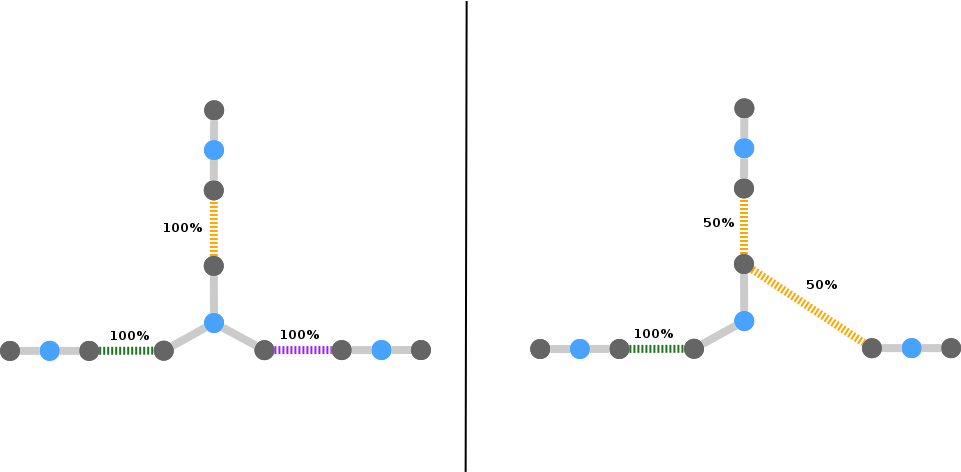
\includegraphics[width=0.56\textwidth]{figures/3modulesvs2}%
	\caption{Link separation capability for an accesspoint with three modules compared to an accesspoints with two modules.}
      }
      \label{fig:3modulesvs2}
    \end{figure}
    
    Compared to the base scenario our link selection and channel assignment algorithm was able to rougly double the throughput with every channel added. 
    Of course this effect is limited by using a separate channel for each link and also by the number of modules for an accesspoint 
    since the former effectively assigns each link its own private channel and the latter is a question of practical relevance as current accesspoints are only 
    shipped with two or a maximum of three radio modules. As our gathered data indicate it is after all an improvement to utilize multiple channels and modules
    compared to AutoWDS basic, but in how far our solution comes in range to a theoretical optimal solution for a given scenario is still an open question.
    
\section{Reflection on the Requirements}
  In this section we analyze by how far we were able to meet the imposed requirements and restrictions.
  
  \subsection{Increased Throughput}
    Our measurement results indicate that throughput could significantly be increased. How much is determined by the input parameters of the algorithms like
    channels that can be utilized and hardware environments like the number of radio modules available at the accesspoints. 
    
  \subsection{Reduced end-to-end Link Failures}
    The survival path property takes care of this requirement. That is for the given error-scenario of one failing connection at a time, there is always
    a backup connection over a different link available as far as the underlying topology permits. As we were not able to test this feature 
    with the given implementation we are nevertheless confident that also this requirement has been met.
    If multi-flow / routing support will be implemented for our hardware in the future a decrease in node separation for failing links should be recognizable.
    Therefore we also met the successfully met the requirement of a two-edge-connected network topology.
    
  \subsection{Multiple Radios Utilized}
    Our algorithm utilizes the radio-modules as far as they are relevant for creating links between accesspoints with a high estimated throughput.
    Depending on the given infrastructure not all radio modules are necessarily used, since not all of them are needed in order to create a connected network topology.
    Moreover using all available links would not be beneficial as the hop distance would decrease but the effective throughput would also decrease by a factor 
    more than the number of participants in that channel.
    
    \begin{figure}[h!]
      \centerline{
	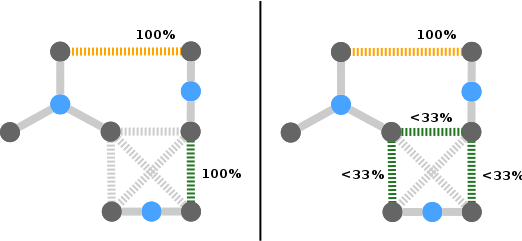
\includegraphics[width=0.56\textwidth]{figures/lessismore}
	\caption{Due to the channel separation and exclusive access to one channel the left scenario is more favourable than the right, 
		  since throughput empirically exponentially decreases and is far below the 33 percent which those links would 
		  have to yield in order to at least provide the same throughput
	}
      }
      \label{fig:lessismore}
    \end{figure}
    
    Having some radio modules to spare gives us the opportunity to use those exclusively for client connections and assigning them a channel which does not interfere with the
    wireless backbone.
    
    \begin{figure}[h!]
      \centerline{
	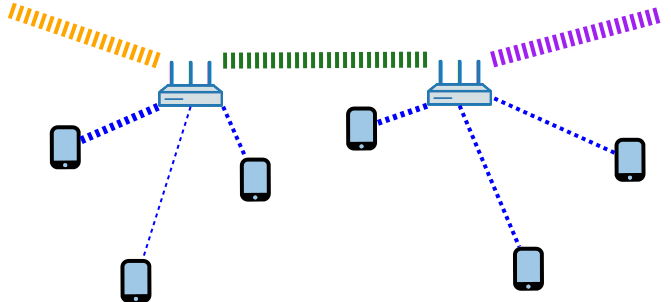
\includegraphics[width=0.56\textwidth]{figures/moduletospare}%
	\caption{Unused Modules used for separate client connections without interfering wlan backbone}
      }
      \label{fig:moduletospare}
    \end{figure}
    
  \subsection{Capability of Using Variable Channelsets}
    Our algorithm selects channels from a given input set of channels. Only those channels are then used to determine the channel assignment.
    It is even possible to specify only one channel, resulting in a topology optimized network graph only.
    Therefore this solution also fullfills this requirement.
    
  \subsection{Centralized Computation and Configuration}
    The requirement dictates that computing a solution should be possible on a centralized entity (Servers/WLC).
    Our algorithm was implemented as a python script and can be run on a single system if given the right input data.
    Creating the configurations for the accesspoint will still be conducted by the central WLC as depicted in \ref{fig:dataflow}.
    
  \subsection{Static Environment} 
    Also the second requirement is taken into consideration, since our algorithm is specially designed for a static environment where link quality 
    and linkstate stay the same for a foreseeable time.
    If major changes in network connectivity or link quality occur the chosen network topology and channel assignment
    may lead to temporal suboptimal results, therefore also a recomputation of the network topology would have to be triggered.
    Currently there are no automatic triggers implemented, but planned in the future.
    
  \subsection{Layer two Usage}
    Accesspoints use bridged point to point connections to span the wireless network backbone, therefore creating no obstacles for layer two frames.
    The ethernet frames are just forwarded like in a switched environment and not encapsulated in layer three packets.
    
  \subsection{Economic Restrictions}
    The Runtime of the algorithms is mainly dependent on the number of connections between the nodes. Calculating the initial spanning tree is done in BFS mode and 
    therefore has quadratic runtime for the worst cast, depending on how sparse the graph is. The following calculation of the survival paths has also quadratic runtime 
    since we iterate over all connections and for each connection in the worst case over all other connections to find the backup path. The channel assignment is then again
    In a common deployment scenario the underlying network graph will be very sparsly connected since the number of accesspoints used and placement are carefully selected.
    Mostly they are placed in a way that they span a network over an area as far as possible.
    Current deployments and deployments in near future won't exceed 100 accesspoints. 
    Even if fully meshed with a total of \(\sum \limits_{i=1}^{100} i = \frac{100(100+1)}{2}=5050\)
    edges it won't pose a problem to the capabilities of a WLC or an administrators machine.
    
\section{Reflection on Related Work}
  Comparing our solution to those of others would need some common ground. For example hardware requirements, number of modules and in general heterogenity/homgenity of
  the network are factor that could play in favor of some algorithms and therefore won't lead to fair results. Additionally different solutions were designed to 
  achieve different goals like throughput, latency or weighted throughput networks. Certainly there we could agree on this common deployment and compare each solution for random
  networks with respect to throughput, but this would require a full-scale simulation as hardware-resources are limited and too easily prone to real world difficulties.
  Although maybe a key aspect of this work, we did not have enough time to simulate even our own solution and therefore neither those of others. Nevertheless we would appreciate
  if someone further work on this field. In order to at least provide some kind of comparison we take a look at the features of each solution.
  
  \subsection{Features of Related Work Systems}
    TODO:
  \subsection{Features of Our System}
    TODO: